\documentclass[12pt]{article}
\usepackage[utf8]{inputenc}
\usepackage{hyperref}
\usepackage{graphicx}
\usepackage[margin=1.2in]{geometry}

\title{Analyzing Fatal Encounters With Police in 2015 Using Nonparametric Methods}
\author{Evan Wagner}
\date{12/14/2021}

\begin{document}

\maketitle

\par \noindent \textbf{Abstract:} We are interested in analyzing data on fatal encounters with police in America in 2015 but cannot assume that our observed values follow a normal distribution. We apply a variety of distribution-free statistical tests to make conclusions about 2015 police killings, comparing each to its normality-assuming counterpart.

\begin{center}
    ***
\end{center}

\tableofcontents


\section{Introduction}

\par In recent years, a spate of high-profile violent encounters with American police officers has focused public attention on such incidents. Media outlets have responded by compiling detailed data on fatal incidents across the U.S. and making it available for statistical analysis. For one, \textit{FiveThirtyEight} compiled data on all such incidents from the year 2015, pulling details of each incident from data gathered by \textit{The Guardian} and adding location-related data from the American Community Survey (ACS) conducted in 2015 by the U.S. Census.\cite{dset} We will attempt to derive statistically significant conclusions from this dataset.

\par \bigskip As shall be seen in the following, the nature of these data prevents us from applying many techniques typically used for statistical analysis. In short, we cannot assume that the populations underlying the parameters we wish to measure are normally distributed, which is a prerequisite for all of the basic techniques taught in beginning statistics courses. Luckily, several savvy statisticians have developed statistical techniques whose conclusions are valid without assuming its parameters follow a distribution, normal or otherwise. We will apply their distribution-free methods to our data on police killings to try and answer several questions of interest.

\par \bigskip Before we begin, two very important hesitations must be addressed. The first is that our conclusions only apply to fatal encounters in the year 2015. With only one year in our sample, we cannot assess the influence of time-based effects on our parameters of interest. Indeed, as police brutality began growing more prominent in the public imagination starting in 2014, it is likely that some police departments have responded to scrutiny of their peacekeeping practices by overhauling them.

\par \bigskip Secondly, our data is not a typical simple random sample (SRS) because it technically includes our entire population of interest: 2015 victims of deadly force. As such, we have no need to estimate means and deviations because we can calculate them directly. That said, our conclusions are still meaningful for comprehending and comparing these data. If a higher power wound back the clock to 2015 and set the conditions back to how they were, we would expect slightly different outcomes due to the contribution of randomness to our parameters. 

\subsection{Data Preparation}

\par In order to apply our techniques, changes were made to the raw data. Rows which contained at least one missing value of a quantitative variable were removed, as were entries labeled \textit{``Unknown"} for some categorical variable; this reduced the number of observations from 467 to 438. Additionally, three new binary variables were created by forming two groups from the levels of categorical variables. The full list of variables is displayed in Table \ref{tab:variables}.

\begin{table}[h]
    \centering
    \begin{tabular}{|l|l|l|l|}
        \hline
        \textbf{Variable} & \textbf{Type} & \textbf{Description} & \textbf{Original Source}\\
        \hline
        $age$ & quantitative & Age of deceased & \textit{The Guardian}\\
        &&&\\
        \hline
        $pop$ & quantitative & Population of tract on which the & U.S. Census\\
        && killing occurred. Tracts are &\\
        && subdivisions of counties containing &\\ && a few thousand residents each. &\\
        \hline
        $share\_white$ & quantitative & Share of tract population that is & U.S. Census\\
        && non-Hispanic white &\\
        \hline
        $share\_black$ & quantitative & Share of tract population that is & U.S. Census\\
        && black (alone, not in combination) &\\
        \hline
        $share\_hispanic$ & quantitative & Share of tract population that is & U.S. Census\\
        && Hispanic/Latino (any race) &\\
        \hline
        $p\_income$ & quantitative & Tract-level median personal income & U.S. Census\\
        && (USD) &\\
        \hline
        $h\_income$ & quantitative & Tract-level median household & U.S. Census\\
        && income (USD) &\\
        \hline
        $county\_income$ & quantitative & County-level median household & U.S. Census\\
        && income (USD) &\\
        \hline
        $comp\_income$ & quantitative & Ratio of $h\_income$ to $county\_income$ & Calculated by\\
        &&& \textit{FiveThirtyEight}\\
        \hline
        $pov$ & quantitative & Tract-level poverty rate (official) & U.S. Census\\
        &&&\\
        \hline
        $urate$ & quantitative & Tract-level unemployment rate & Calculated by\\
        &&& \textit{FiveThirtyEight}\\
        \hline
        $college$ & quantitative & Share of tract population $\ge$ 25 years & Calculated by\\
        && old with BA or higher & \textit{FiveThirtyEight}\\
        \hline
        \hline
        $gender$ & categorical & Gender of deceased & \textit{The Guardian}\\
        \hline
        $raceethnicity$ & categorical & Race/ethnicity of deceased & \textit{The Guardian}\\
        \hline
        $cause$ & categorical & Cause of death & \textit{The Guardian}\\     \hline
        $armed$ & categorical & How/whether deceased was armed & \textit{The Guardian}\\
        \hline
        $county\_bucket$ & categorical & Tract-level household income, & Calculated by\\
        && quintile within county & \textit{FiveThirtyEight}\\
        \hline
        $nat\_bucket$ & categorical & Tract-level household income, & Calculated by\\
        && quintile nationally & \textit{FiveThirtyEight}\\
        \hline
        \hline
        $white$ & binary & Coded 1 when $raceethnicity =$ & Computed by\\
        && $``White"$, 0 otherwise & the author\\
        \hline
        $male$ & binary & Coded 1 when $gender = ``Male"$, & Computed by\\
        && 0 when $gender = ``Female"$ & the author\\
        \hline
        $armedyes$ & binary & Coded 0 when $armed = ``No"$, & Computed by\\
        && 1 otherwise & the author\\
        \hline
    \end{tabular}
    \caption{Variables in the dataset}
    \label{tab:variables}
\end{table}


\section{Two-Sample Tests}

\par If we split a quantitative variable into two groups based on a binary variable, we can test whether the two samples have equal medians and/or variance. Box plots were generated for each of the possible variable choices to identify potential differences. The author selected three pairings of variables whose boxplots  seemed to show significantly different medians, shown in Figure \ref{fig:twosample_boxplots} along with histograms to give the reader a sense of the distribution's shape. We see that each distribution is somewhat right-skewed, and the white age distribution seems skinnier than the non-white distribution in the first histogram.

\begin{figure}[h]
    \centering
    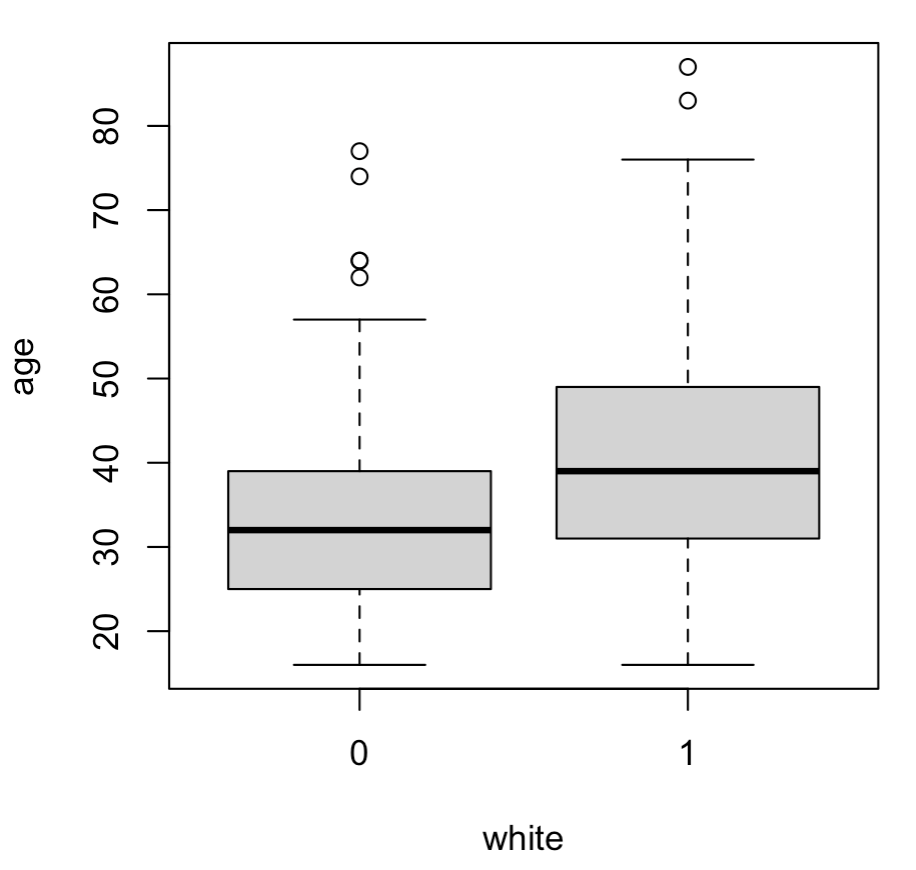
\includegraphics[scale=.3]{boxplot_age_white.png}
    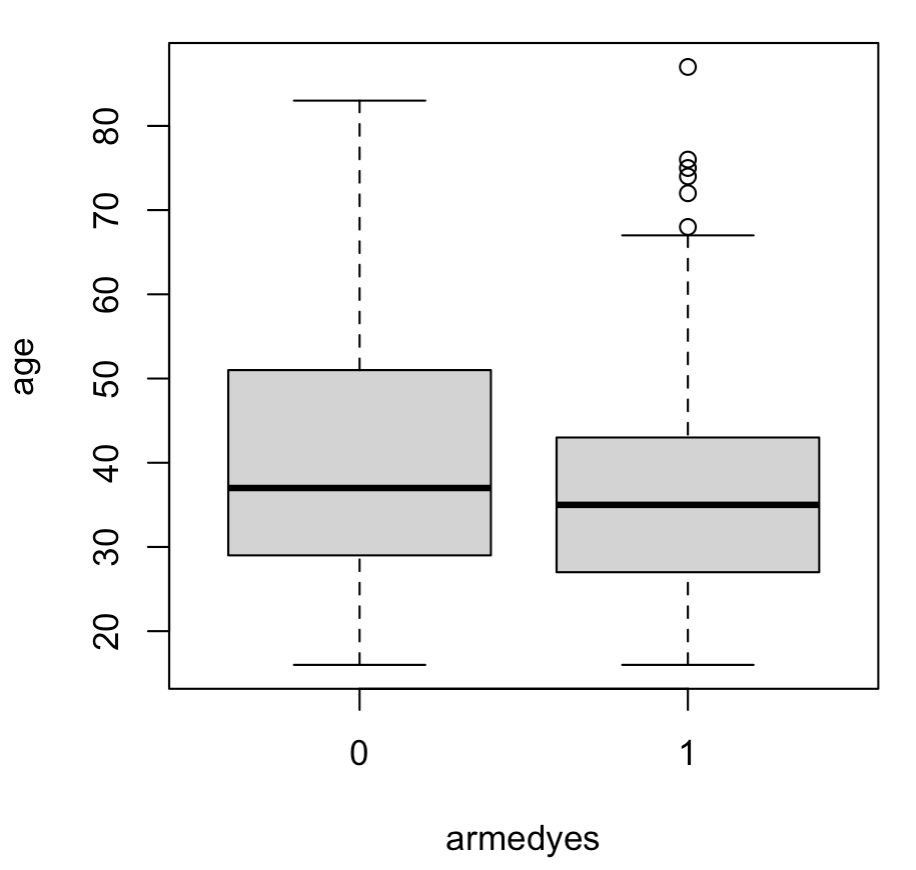
\includegraphics[scale=.3]{boxplot_age_armedyes.png}
    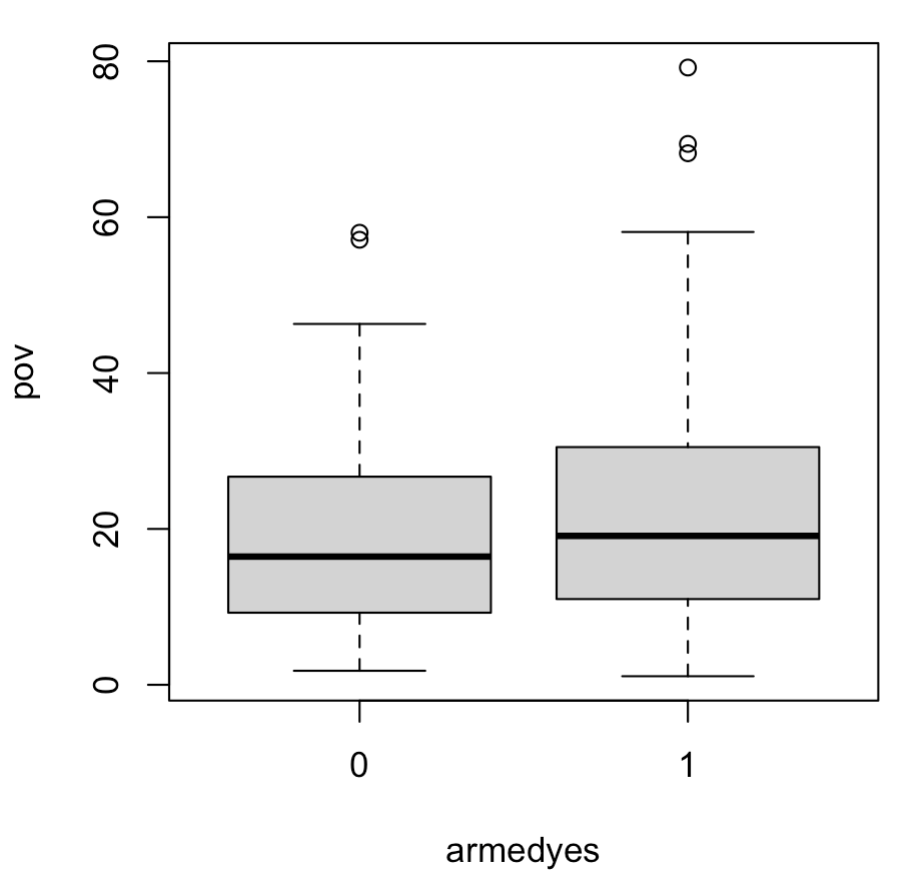
\includegraphics[scale=.3]{boxplot_pov_armedyes.png}
    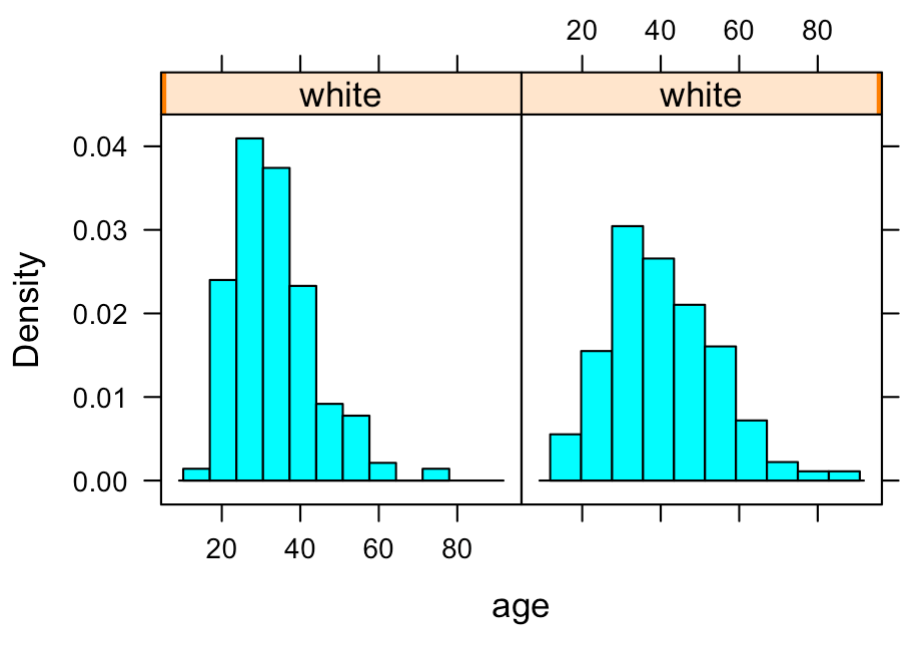
\includegraphics[scale=.3]{histplot_age_white.png}
    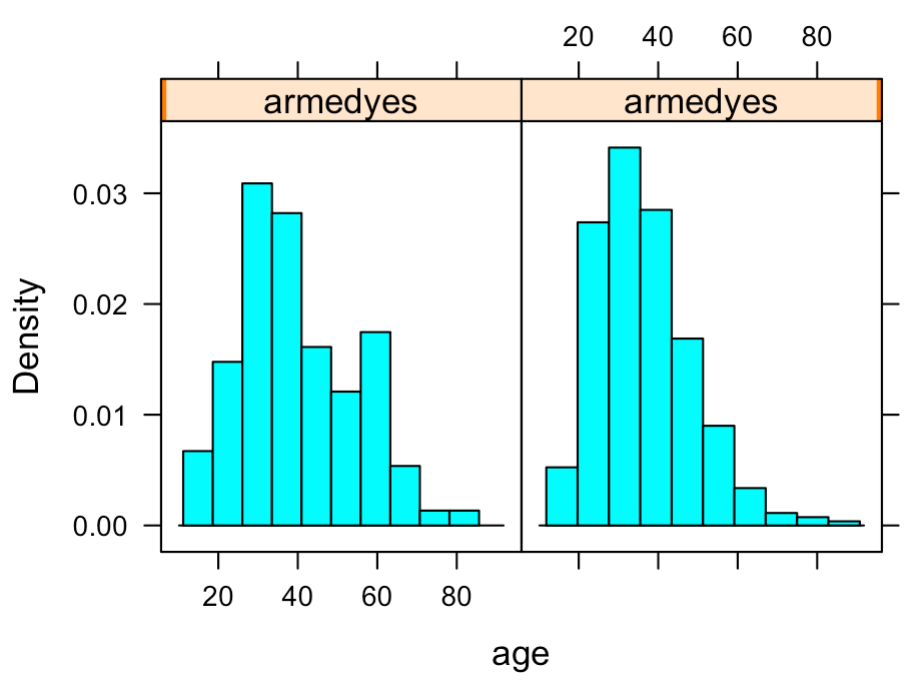
\includegraphics[scale=.3]{histplot_age_armedyes.png}
    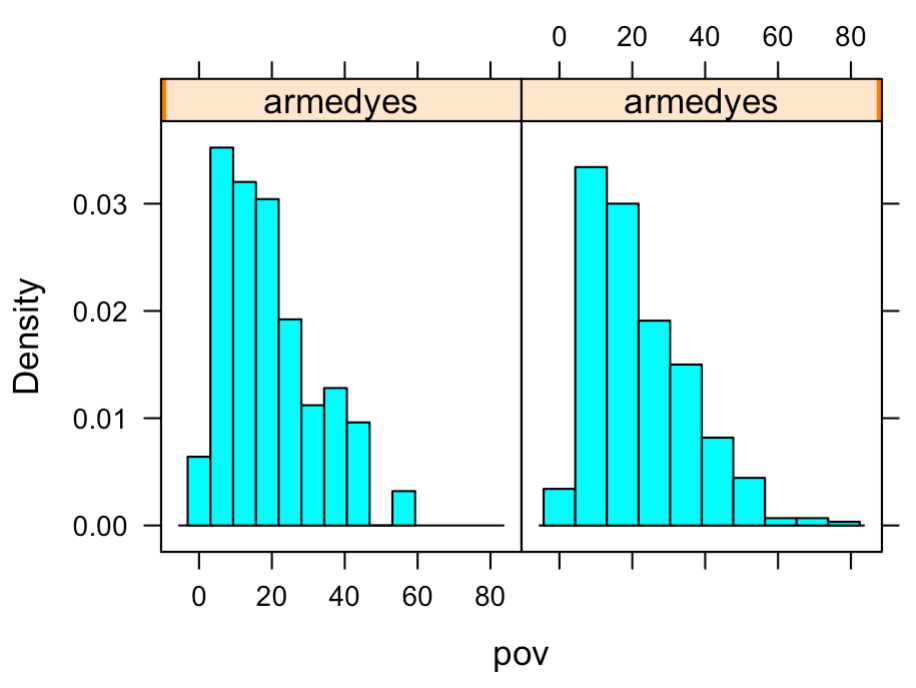
\includegraphics[scale=.3]{histplot_pov_armedyes.png}
    \caption{Box plots and histograms of three quantitative-binary variable pairs }
    \label{fig:twosample_boxplots}
\end{figure}

\subsection{Age vs. Whiteness: Parametric Analysis}

\par Our data includes 229 white victims and 209 nonwhite victims. In order to find a significant difference between the average age of these two populations, our first instinct might be to conduct a $t$-test. Let $\mu_W$ be the mean age of white victims and $\mu_N$ be the mean of nonwhite victims. Our null hypothesis is that these two means are equal, or equivalently, their difference $\mu_W - \mu_N = 0$. Our estimate of the difference is simply the difference in the mean ages of our two samples, which turns out to be 7.259 years.

\par \bigskip But is this difference significant? Using the base R function \texttt{t.test()}, we obtain a $p$-value of $1.038*10^{-9}$ and a 95 percent confidence interval of $(4.973, 9.544)$. If this test were valid, we would reject the null hypothesis and declare with 95 percent confidence that white victims are between 4.973 and 9.544 years older than nonwhite victims on average.

\par \bigskip Unfortunately, a quick look at some diagnostic plots shows us that the conditions for inference based on the $t$-test are not met. Figure \ref{fig:ttest1_plots} shows a plot of the residuals vs. fitted values from our model,\footnote{To create the plots in Figures \ref{fig:ttest1_plots} and \ref{fig:ttest2_plots}, the author used one-way ANOVA tests, which in the two-sample case are equivalent to $t$-tests.} as well as a normal probability plot of the residuals. The residuals for the nonwhite population seem to be less widely distributed than for the white population, calling the equal variance assumption into question. We can further test for unequal variance with Levene's test. Using the R function \texttt{levene.test()} from the package \texttt{lawstat}, we obtain a $p$-value of .000413 and conclude that the variances of the two populations are indeed unequal.

\vspace{.2in}

\begin{figure}[h]
    \centering
    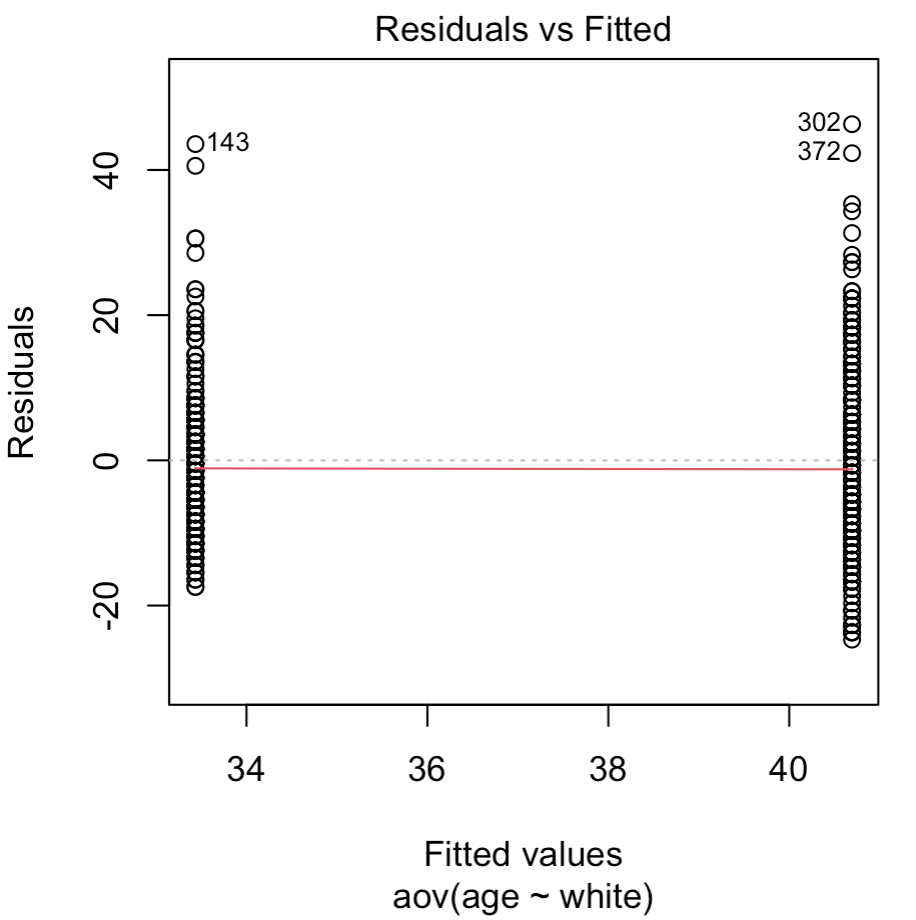
\includegraphics[scale=.4]{ttest1_plot1.png}
    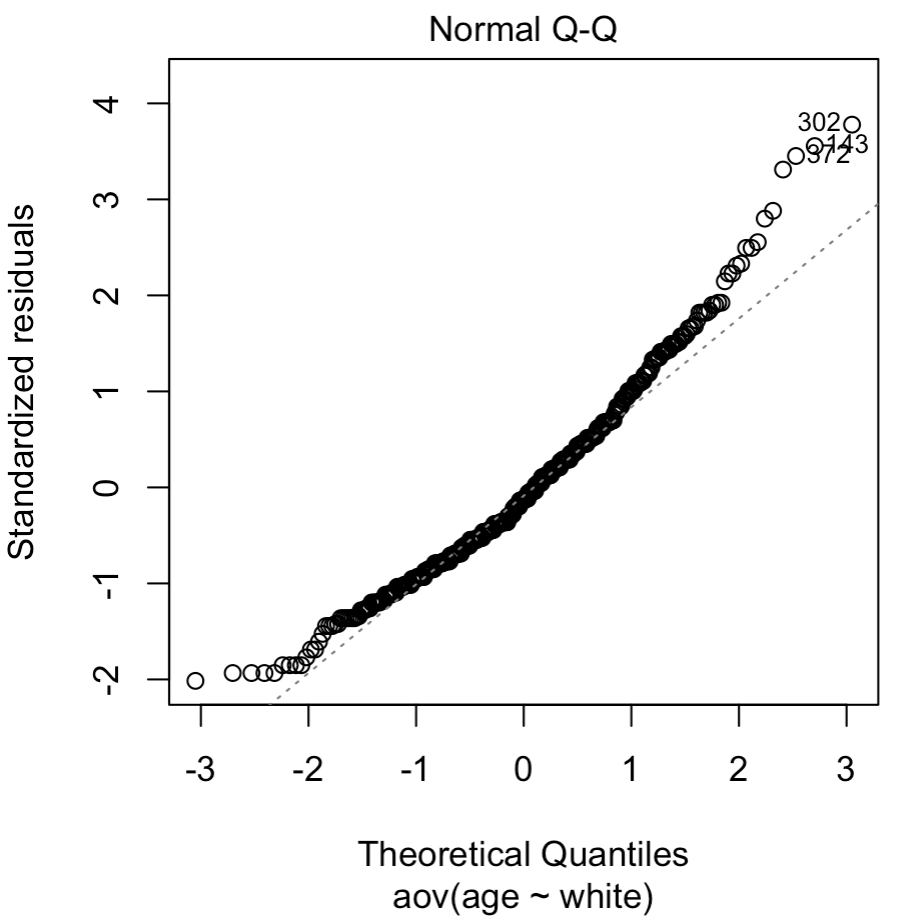
\includegraphics[scale=.4]{ttest1_plot2.png}
    \caption{Diagnostic plots for the two-sample $t$-test of $age$ vs. $white$}
    \label{fig:ttest1_plots}
\end{figure}

\par \bigskip Furthermore, we have evidence that our populations are not distributed normally. The normal probability plot shows residuals that depart strongly from the expected normal curve at both tails. We can also conduct the Anderson-Darling test for normality. Using the R function \texttt{ad.test()} from the package \texttt{nortest}, we obtain a $p$-value of $1.013*10^{-7}$ and conclude that our residuals do not follow the normal distribution. Clearly, any inference we make from the standard $t$-test on these two samples would be invalid.

\newpage

\par \bigskip Perhaps a transformation on $age$ will satisfy the conditions for the $t$-test. In Figure \ref{fig:ttest1_plots} we see upper outliers in the boxplots and a right skew in the histograms. The square root of age might have a more symmetric distribution. Sure enough, our plots of $\sqrt{age}$ vs. $white$ and the new $t$-test residuals (shown in Figure \ref{fig:ttest1_transformed_plots}) depict a distribution that looks much closer to the normal curve. However, Levene's test of the transformed variance returns a $p$-value of 0.00844, and the Anderson-Darling test returns a $p$-value of 0.0396. We still reject their null hypotheses of equally-varying and normal residuals.

\begin{figure}[h]
    \centering
    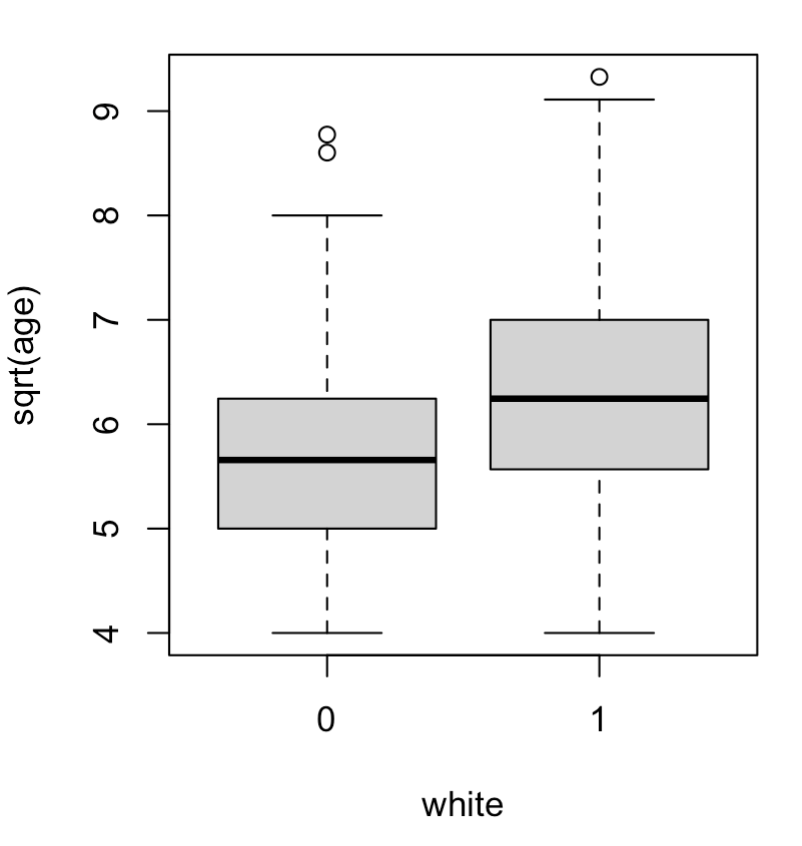
\includegraphics[scale=.4]{boxplot_sqrtage_white.png}
    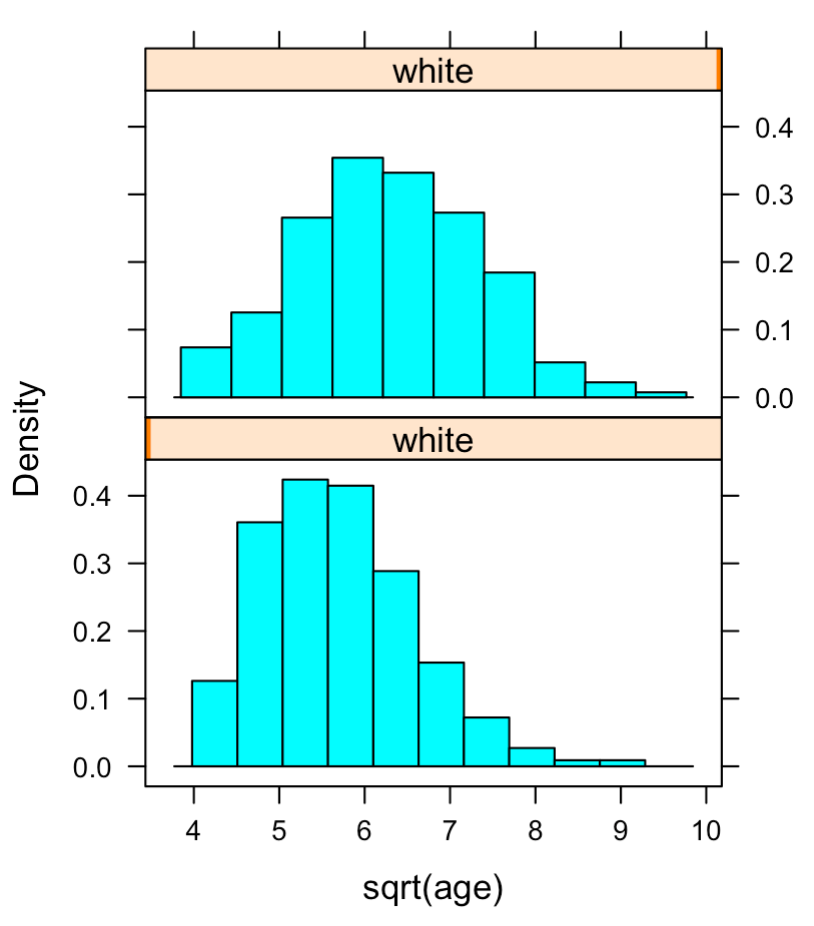
\includegraphics[scale=.4]{histplot_sqrtage_white.png}
    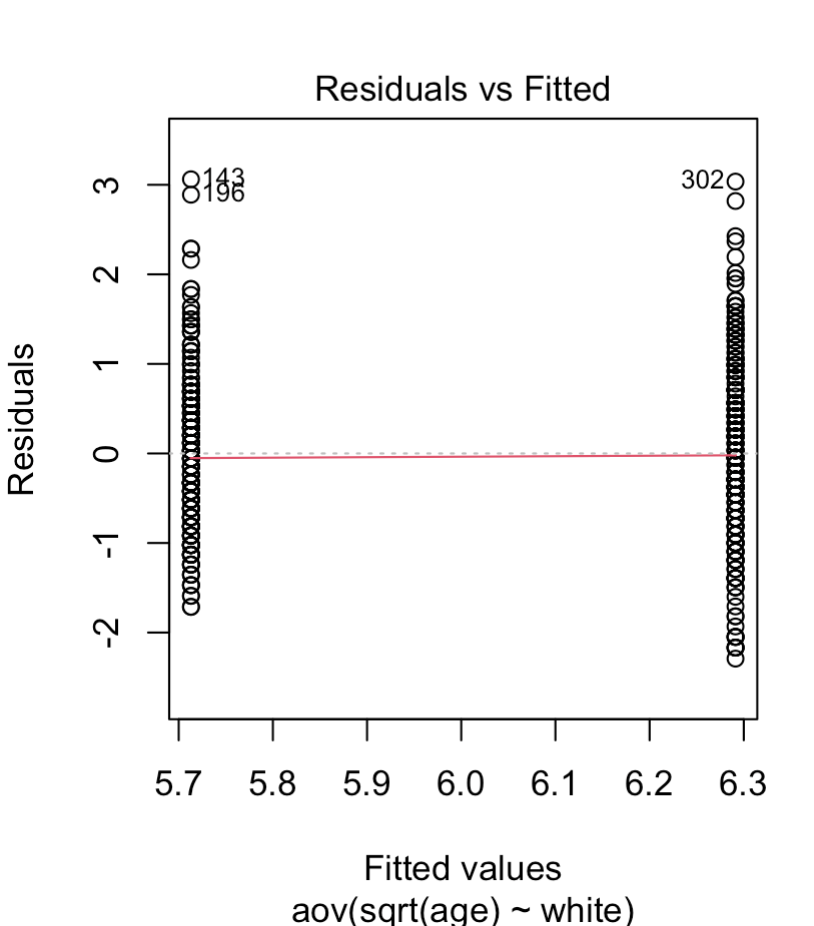
\includegraphics[scale=.4]{ttest1_transformed_plot1.png}
    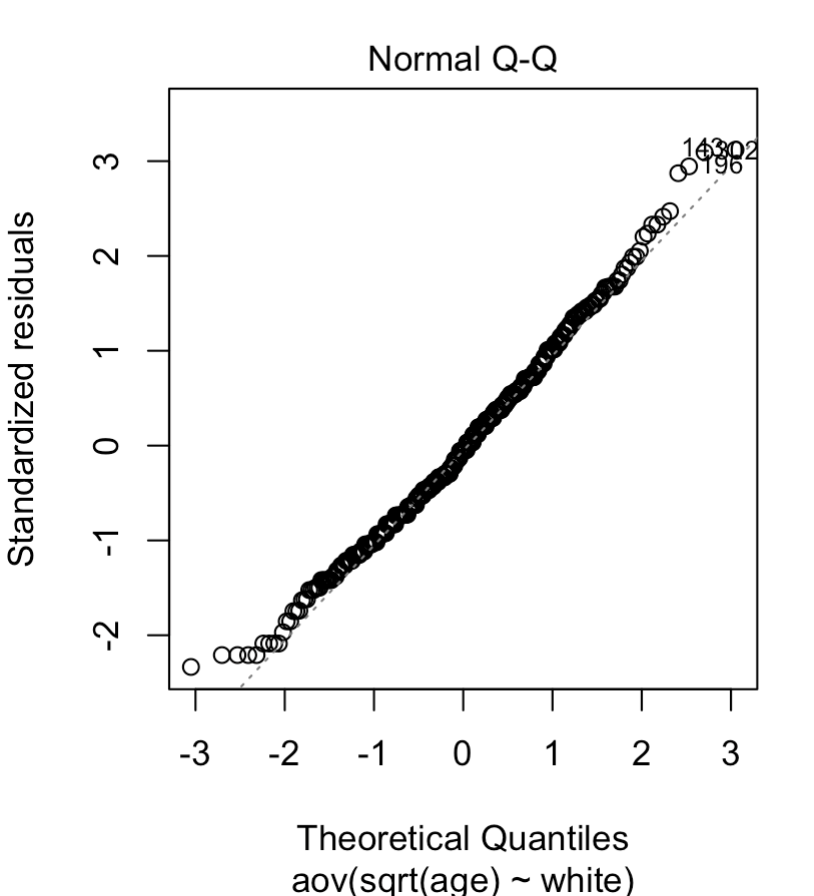
\includegraphics[scale=.4]{ttest1_transformed_plot2.png}
    \caption{Plots of $\sqrt{age}$ vs. $white$}
    \label{fig:ttest1_transformed_plots}
\end{figure}

\par For the sake of comparison with our nonparametric procedures, we convert the estimates from the $t$-test on $\sqrt{age}$ against $white$ back into regular years and report them. Though their distribution is still invalid for the $t$-test, it is an improvement on the untransformed model and its conclusions are slightly more representative of the truth. Our new $p$-value is $1.381*10^{-9}$. Our new estimate is the difference between the squared estimates of mean $\sqrt{age}$, which comes out to 6.941. We form the new confidence interval by taking the squared mean $\sqrt{age}$ of white victims and subtracting the squared difference between the mean $\sqrt{age}$ of white victims and the lower bound of our confidence interval, then doing the same with the upper bound. This new interval is $(4.810, 9.004)$.

\par \bigskip In light of the problematic distribution of age against whiteness, we turn to nonparametric methods for a more robust analysis of the two variables.

\subsection{Age vs. Whiteness: Nonparametric Analysis}

\par \bigskip We will first determine whether the distributions underlying our two populations are dispersed equally. Setting $\gamma^2 = \frac{var({\sqrt{age}}_{white})}{var({\sqrt{age}}_{nonwhite})}$, we seek to determine whether the ratio of the two population variances $\gamma^2$ is significantly far from 1 in either direction.

\par \bigskip Our result from Levene's test suggests that these variances are unequal. However, we see from Figure \ref{fig:ttest1_plots} that the data contains several outliers, to which Levene's test is very sensitive. In comparison, the Miller jackknife procedure is much more resilient to outliers because its test statistic is adjusted based on the contribution of each observation to the overall mean. We can make a more robust conclusion about the variances of these two populations by applying the jackknife procedure.

\bigskip \textbf{Miller jackknife test}

\bigskip $H_0: \gamma^2 = 1$

$H_3: \gamma^2 \not= 1$ \hspace{1in} Reject $H_0$ if $|Q| \ge z_{\alpha/2}$.

\par \bigskip Using the custom R function \texttt{jackKnife()}, we find that $Q = 2.420$ and obtain a $p$-value of 0.00777, which is quite similar to that of Levene's test. We also obtain an estimate for the ratio between the variances of the populations, $\bar{\gamma}^2 = 1.581$, and the associated 95 percent confidence interval $(1.141, 2.191)$. In other words, we are 95 percent confident that the variance in age for white victims is between 1.141 and 2.191 times larger than that of nonwhite victims.

\par \bigskip Now we move on to determining whether the median ages are different for our two populations. In light of our rejection of the null hypothesis with the Miller jackknife, we should conduct the Fligner-Policello test, which does not assume equality of variance. We need not transform and untransform $age$ for this test: it is based on the ranks of observations relative to each other, and since the square root is an increasing function, it does not change the rankings of observations at all. Therefore, the test will not conclude anything differently before and after transformation. Additionally, since our sample has many observations and because it reduces computing time greatly, we will use the large-sample approximation (LSA) of the Fligner-Policello test.

\bigskip \textbf{Fligner-Policello test}

\bigskip $H_0: \theta_{white} = \theta_{nonwhite}$

$H_3: \theta_{white} \not= \theta_{nonwhite}$ \hspace{1in} Reject $H_0$ if $|\hat{U}| \ge z_{\alpha/2}$.

\par \bigskip Using the R function \texttt{pFligPoli()} from the package \texttt{NSM3}, we find that $\hat{U} = 6.353$ and obtain a $p$-value of $2.112*10^{-10}$. Thus we reject the null hypothesis and conclude that the median age of white victims is different than that of non-white victims.

\par \bigskip For an estimate of the true difference in median $\theta_{white} - \theta_{nonwhite}$, we can use the Hodges-Lehmann $\hat{\Delta}$, which is the median of the differences between each measurement of $age_{nonwhite}$ and $age_{white}$. Using the base R function \texttt{wilcox.test()}, we see that $\hat{\Delta} = 7.000$. In other words, we estimate that white victims are roughly 7 years younger than nonwhite victims on average. The output also finds a confidence interval of $(5.000, 9.000)$, but that is meaningless if the variances of our populations are unequal.

\par \bigskip Table \ref{tab:twosample1_results} summarizes the results obtained from our tests of age broken down by whiteness. It appears that the true difference in means (and our sample size) is large enough to make the conclusions of these tests very similar. 

\vspace{.2in}

\begin{table}[h]
    \centering
    \begin{tabular}{|l|c|c|c|c|}
        \hline
        \textbf{parameter} & \textbf{procedure} & \textbf{p-value} & \textbf{estimate} & \textbf{95 pct. CI}\\
        \hline
        Location & $t$-test & $1.381*10^{-9}$ & $\hat{\mu}_W-\hat{\mu}_N = 6.941$ & $(4.810, 9.004)$\\
        & Fligner-Policello & $2.111*10^{-10}$ & $\hat{\Delta} = 7.000$ & not meaningful\\
        \hline
        Dispersion & Levene's test & 0.00844 & -- & --\\
        & Miller jackknife & 0.00777 & $\bar{\gamma}^2 = 1.396$ & $(1.065, 1.829)$\\
        \hline
    \end{tabular}
    \caption{Results for $age$ vs. $white$}
    \label{tab:twosample1_results}
\end{table}

\subsection{More Two-Sample Analysis}

\par For the remainder of the paper, we will continue applying a square root to $age$ and all other quantitative variables, as it improves conditions in every case.

\par \bigskip Our second analysis, of age broken down by whether or not the victim was armed, goes quite similarly to our first. There are 338 armed and 100 unarmed victims in the dataset. This time, the Anderson-Darling test still rejects the normality condition, but Levene's test returns a $p$-value of 0.0850, hovering right on the brink of the common significance level of $\alpha = 0.05$. The Miller jackknife returns a similar $p$-value of 0.0584. Therefore, in addition to the Fligner-Policello test, we proceed with the Wilcoxon rank sum test using \texttt{wilcox.test()} and obtain a meaningful 95 percent confidence interval for the difference in population medians $\theta_{A}-\theta_{U}$. Though both nonparametric tests for unequal means are less certain than the $t$-test, they still reject the null at alpha levels .05 and higher. Full results are shown in Table \ref{tab:twosample2_results}.

\begin{table}[h]
    \centering
    \begin{tabular}{|l|c|c|c|c|}
        \hline
        \textbf{parameter} & \textbf{procedure} & \textbf{p-value} & \textbf{estimate} & \textbf{95 pct. CI}\\
        \hline
        Location & $t$-test & 0.0328 & $\hat{\mu}_U-\hat{\mu}_A = -3.274$ & $(-6.403, -0.266)$\\
        & rank sum & 0.0400 & $\hat{\Delta} = -3.000$ & $(-6.000, -0.0000587)$\\
        & Fligner-Policello & 0.0454 & -- & --\\
        \hline
        Dispersion & Levene's test & 0.0850 & -- & --\\
        & Miller jackknife & 0.0584 & $\bar{\gamma}^2 = 0.709$ & (0.574, 1.010)\\
        \hline
    \end{tabular}
    \caption{Results for $age$ vs. $armedyes$}
    \label{tab:twosample2_results}
\end{table}

\par As for $pov$ vs. $armedyes$, normal residuals are again soundly rejected, but neither variance test could conclude that the populations have different scales. We proceed only with the Wilcoxon rank sum test, which fails to find a difference in medians. Therefore, we do not have sufficient evidence to conclude that the populations are distributed differently in any way. In this case, we see that the rank sum test is slightly less confident than the $t$-test, while the Miller jackknife is more confident than Levene's test. Full results are shown in Table \ref{tab:twosample3_results}.

\begin{table}[h]
    \centering
    \begin{tabular}{|l|c|c|c|c|}
        \hline
        \textbf{parameter} & \textbf{procedure} & \textbf{p-value} & \textbf{estimate} & \textbf{95 pct. CI}\\
        \hline
        Location & $t$-test & 0.1483 & $\hat{\mu}_A-\hat{\mu}_U = 2.009$ & $(-0.749, 4.568)$\\
        & rank sum & 0.1657 & $\hat{\Delta} = 1.800$ & $(-0.800, 4.400)$\\
        \hline
        Dispersion & Levene's test & 0.6036 & -- & --\\
        & Miller jackknife & 0.3010 & $\bar{\gamma}^2 = 1.078$ & $(0.814, 1.427)$\\
        \hline
    \end{tabular}
    \caption{Results for $pov$ vs. $armedyes$}
    \label{tab:twosample3_results}
\end{table}


\section{One-Way Analysis of Variance Methods}

\par In the previous section, we found a significant race-based difference in the ages of deadly force victims between two racial categories, white and nonwhite. In the parametric setting, we could extend our analysis to more than two categories using a one-way analysis of variance (ANOVA) model, then make comparisons between each difference with Tukey's honest significant differences (HSD). This section explores the analogous distribution-free tests: the Kruscal-Wallis test for unequal treatment effects, and the Steel, Dwass, Critchlow-Fligner multiple comparisons procedure.

\subsection{Age vs. Race: Parametric Analysis}

\begin{table}[h]
    \centering
    \begin{tabular}{|c|c|c|c|c|}
        \hline
        ``White" & ``Black" & ``Hispanic/Latino" & ``Asian/Pacific Islander" & ``Native American"\\
        229 & 131 & 64 & 10 & 4\\
        \hline
    \end{tabular}
    \caption{Observation counts for the five levels of $raceethnicity$}
    \label{tab:raceethnicity_levels_n}
\end{table}

\par Table \ref{tab:raceethnicity_levels_n} shows the count of observations for the five levels of $raceethnicity$. The last two groups have only 10 and 4 observations, respectively, making them too much smaller than the other three for valid comparisons. Thus we drop observations coded ``Asian/Pacific Islander" and ``Native American" and compare the remaining three.

\begin{figure}[h]
    \centering
    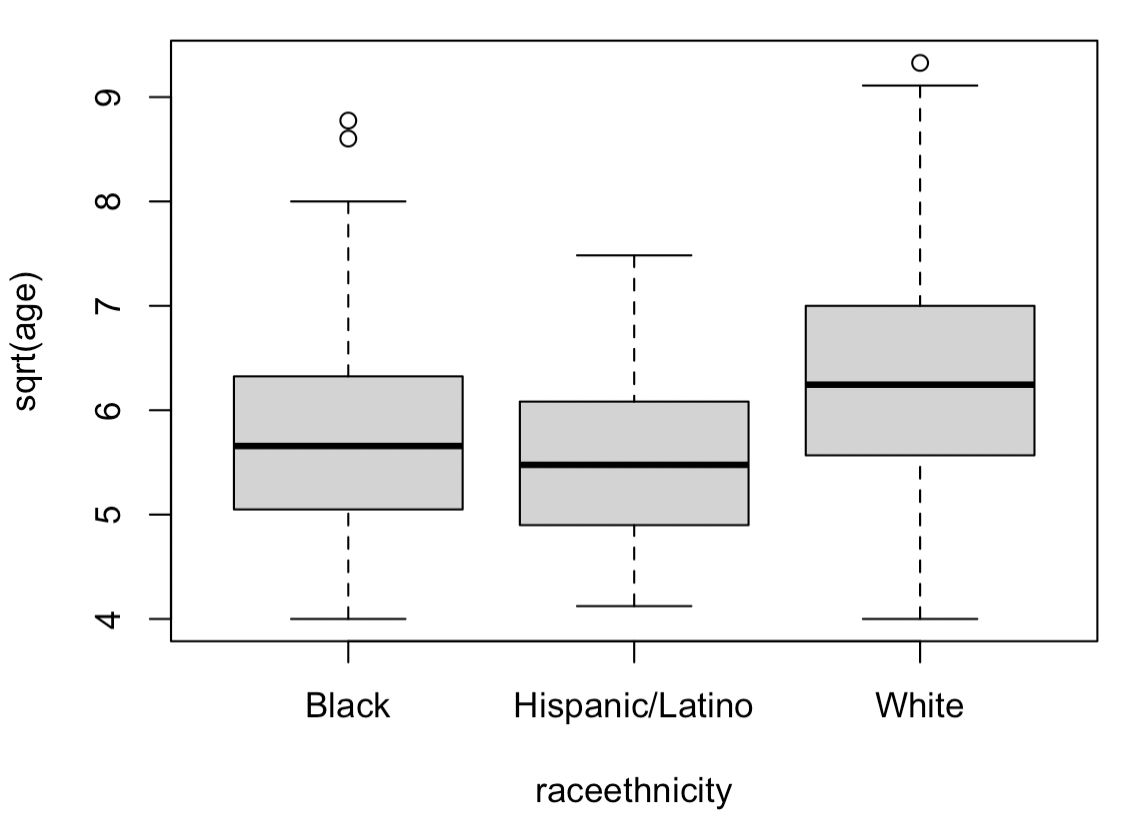
\includegraphics[scale=.4]{boxplot_sqage_raceethnicity.png}
    \caption{Box plots of $\sqrt{age}$ vs. three levels of $raceethnicity$}
    \label{fig:aov1_boxplots}
\end{figure}

\par We see in Figure \ref{fig:aov1_boxplots} that the median $\sqrt{age}$ of white victims looks significantly higher than for both Black and Latino victims. Using the base R function \texttt{aov()}, we fit an ANOVA model to the data and obtain a $p$-value of $4.273*10^{-9}$. If this test were valid, we would conclude quite confidently that at least one of the treatment effects $\tau_{W}, \tau_{B}, \tau_{L}$ is not equal to the rest.

\par \bigskip We would then proceed with a multiple comparisons procedure, such as Tukey's HSD. Using the base R function \texttt{TukeyHSD()}, we obtain intervals for the three configurations of differences in means, adjusted for differences in variance, with 95 percent overall confidence. As shown in Table \ref{tab:aov1_results}, Tukey's HSD claims that, on average, white victims are older than both Black and Latino victims.

\par \bigskip These distribution-reliant claims ring hollow when we check their conditions for inference. Shown in Figure \ref{fig:aov1_plots}, the residuals appear to have different-sized variances for the three groups and lift up considerably from the tails of the expected normal distribution. The picture gets more complicated when we conduct statistical tests: though Levene's test returns a $p$-value of .0243, the Anderson-Darling test yields a $p$-value of 0.0564, which rejects the null hypothesis of normality only at a weak significance level of 0.1. We may consider the ANOVA model somewhat more meaningful in this case, but our distribution-free methods will give us much more robust conclusions.

\vspace{.2in}

\begin{figure}[h]
    \centering
    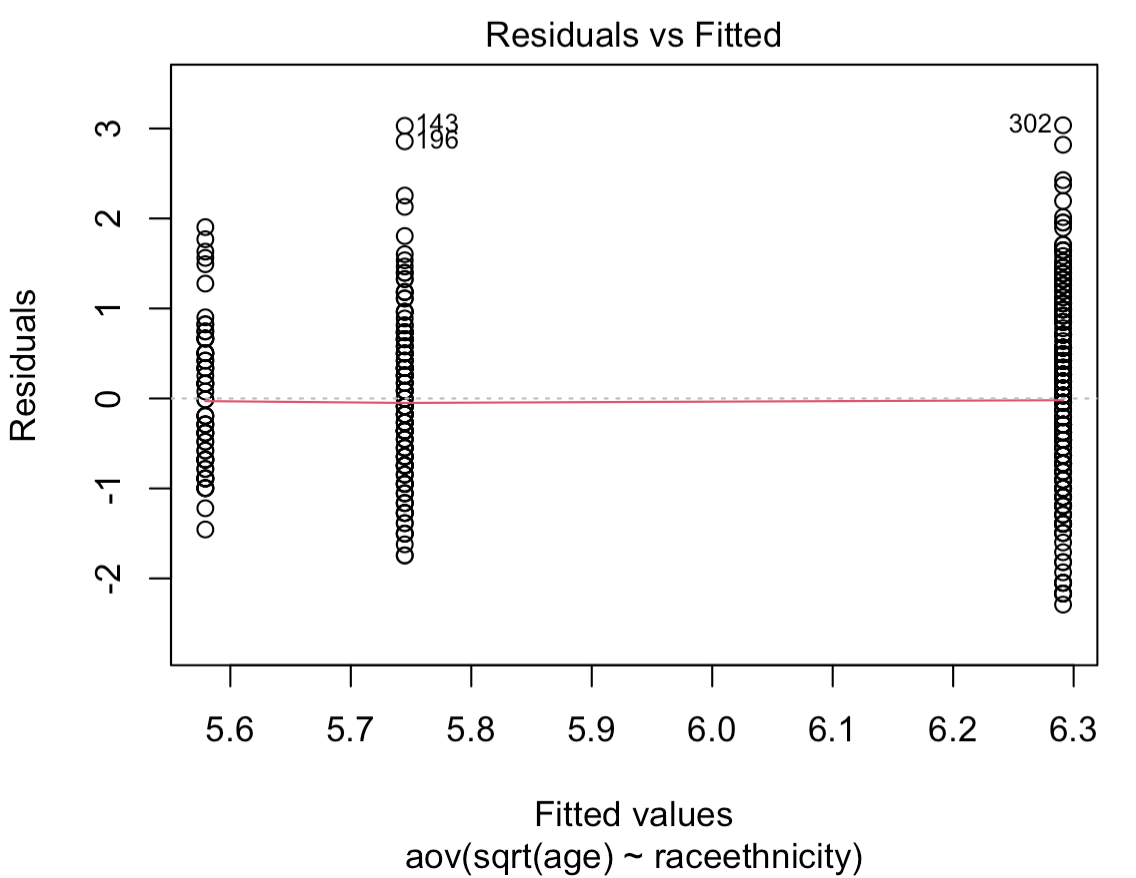
\includegraphics[scale=.35]{aov1_plot1.png}
    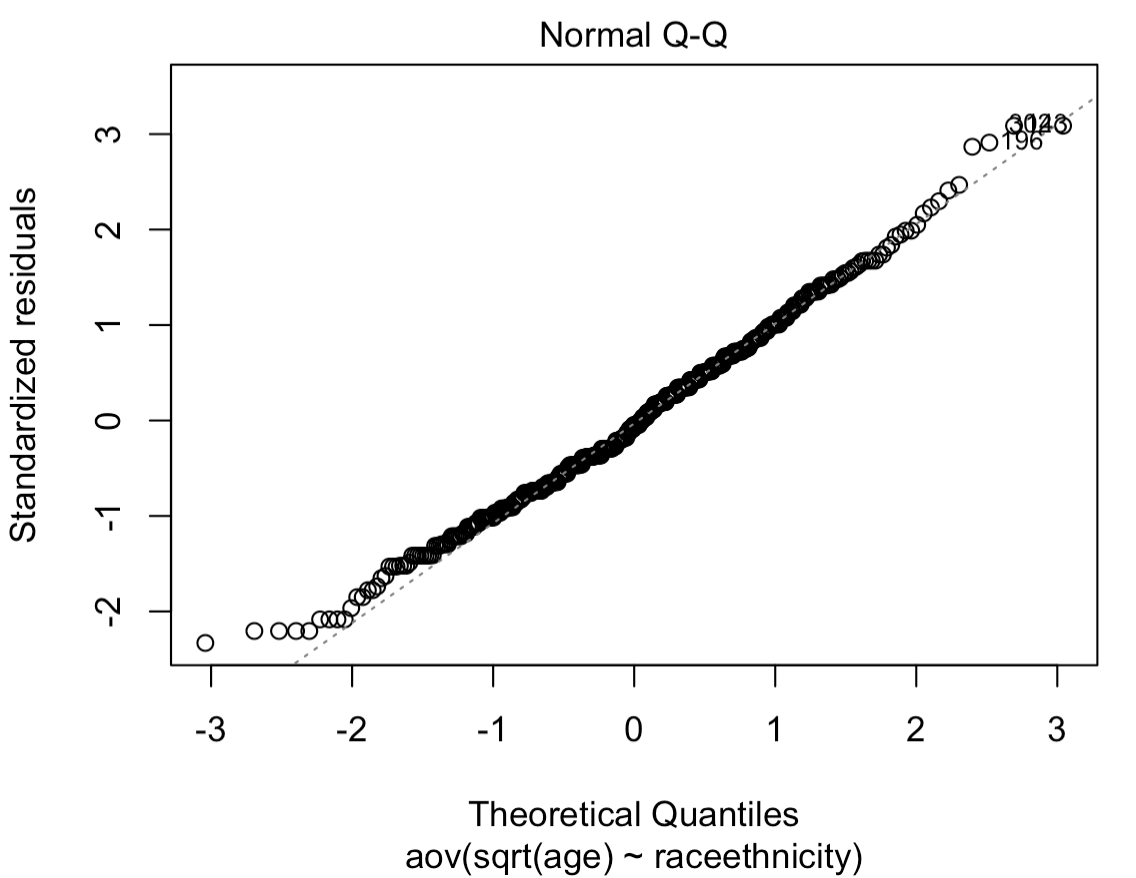
\includegraphics[scale=.35]{aov1_plot2.png}
    \caption{Diagnostic plots for the ANOVA model of $age$ vs. $raceethnicity$}
    \label{fig:aov1_plots}
\end{figure}

\subsection{Age vs. Race: Nonparametric Analysis}

\par Turning to our nonparametric toolbox, we apply the Kruscal-Wallis test, which ranks the combined samples to measure whether the observations in at least one of them are generally ranked higher or lower than those of the other two samples. This test assumes the populations of interest have equal variance, so its results are questionable considering the rejection of the null hypothesis of Levene's test. That said, it is much more resilient to unequal variance than the ANOVA model, so its conclusions are more robust. We will once again perform this rank-based test on the untransformed $age$ variable and use the LSA to reduce computing time.

\newpage

\textbf{Kruscal-Wallis test}

\bigskip $H_0: \tau_{W} = \tau_{B} = \tau_{L}$

$H_1:$ Not all $\tau_k$ equal, $k \in \{W,B,L\}$ \hspace{.5in} Reject $H_0$ if $H^{\prime} \ge \chi^2_{2,\alpha}$.

\par \bigskip Using the R function \texttt{pKW()} from the package \texttt{NSM3}, we find that $H^{\prime} = 37.515$ and obtain a $p$-value of $7.140*10^{-9}$. We reject the null hypothesis and conclude that at least one of the three groups has a different median age than at least one of the others. Note that the Kruscal-Wallis $p$-value is only marginally higher than that of the ANOVA model, and both firmly reject the null hypothesis.

\par \bigskip Our conclusion from the Kruscal-Wallis test motivates us to identify significant pairwise differences with the Steel-Dwass-Critchlow-Fligner procedure, which applies the rank sum test to the three configurations of combined pairs of populations while maintaining overall confidence of $1-\alpha$.

\bigskip \textbf{Steel, Dwass, Critchlow-Fligner procedure}

\bigskip For each pair $(\tau_u,\tau_v)$, decide $\tau_u \not= \tau_v$ if $|W^*_{uv}| \ge w^*_{\alpha}$.

\par \bigskip Using the R function \texttt{pSDCFlig()} from the package \texttt{NSM3}, we obtain the three statistics $W^*_{uv}$ and use the LSA. Based on its results (shown in Table \ref{tab:aov1_results}), we decide with 95 percent overall confidence that white victims have a different median age than Black and Latino victims. We can now use a procedure devised by Spjøtvoll to find adjusted Hodges-Lehmann estimators for each difference in group medians. Using custom R code, we obtain the estimates $\hat{\theta}_{WB} = 6.849$ and $\hat{\theta}_{WL} = 8.309$; the estimate $\hat{\theta}_{BL} = 1.460$ is not significant. Finally, from the ordered differences of each population, we find three intervals for the true median with 95 percent overall confidence.

\par \bigskip The results of this subsection are summarized in Table \ref{tab:aov1_results}. We see that our nonparametric methods yield $p$-values that are about twice the size of the parametric $p$-values, except for the test of $\theta_{BL}$, which is slightly smaller than its distribution-based counterpart. That said, every conclusion is quite strong in this case, and the outcomes of the two types of tests are no different. 

\vspace{.2in}

\begin{table}[h]
    \centering
    \begin{tabular}{|l|c|c|c|c|}
        \hline
        \textbf{parameter} & \textbf{procedure} & \textbf{p-value} & \textbf{estimate} & \textbf{95 pct. CI}\\
        \hline
        General & one-way ANOVA & $4.273*10^{-9}$ & -- & --\\
        differences & Kruscal-Wallis & $7.140*10^{-9}$  & -- & --\\
        \hline
        $\theta_{WB}$ & Tukey's HSD & 0.0000019 & $\hat{\mu}_{WB} = 6.577$ & $(3.595, 9.430)$\\
        & SDCFlig & 0.0000038 & $\hat{\theta}_{WB} = 6.849$ & $(4.000, 10.000)$\\
        \hline
        $\theta_{WL}$ & Tukey's HSD & 0.0000015 & $\hat{\mu}_{WL} = 8.452$ & $(4.687, 12.001)$\\
        & SDCFlig & 0.0000022 & $\hat{\theta}_{WL} = 8.309$ & $(5.000, 12.000)$\\
        \hline
        $\theta_{BL}$ & Tukey's HSD & 0.5137 & $\hat{\mu}_{BL} = 1.874$ & $(-2.132, 5.521)$\\
        & SDCFlig & 0.4601 & $\hat{\theta}_{BL} = 1.460$ & $(-2.000, 5.000)$\\
        \hline
    \end{tabular}
    \caption{Results for $age$ vs. $raceethnicity$}
    \label{tab:aov1_results}
\end{table}

\newpage

\subsection{More One-Way Analysis}

We proceed with three additional analyses of treatment effects with the same methods.

\begin{figure}[h]
    \centering
    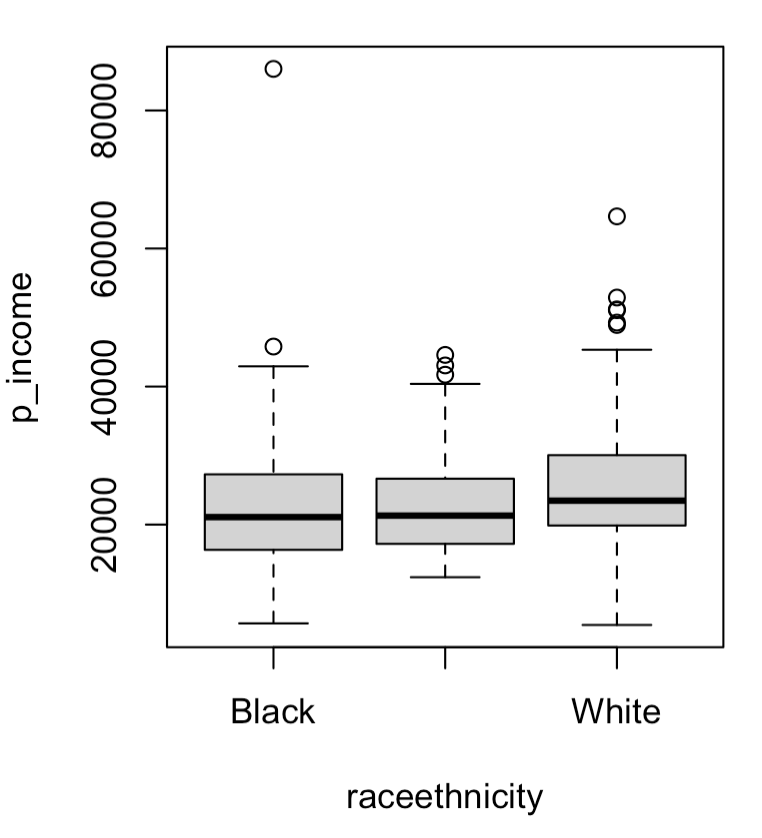
\includegraphics[scale=.35]{boxplot_pincome_race.png}
    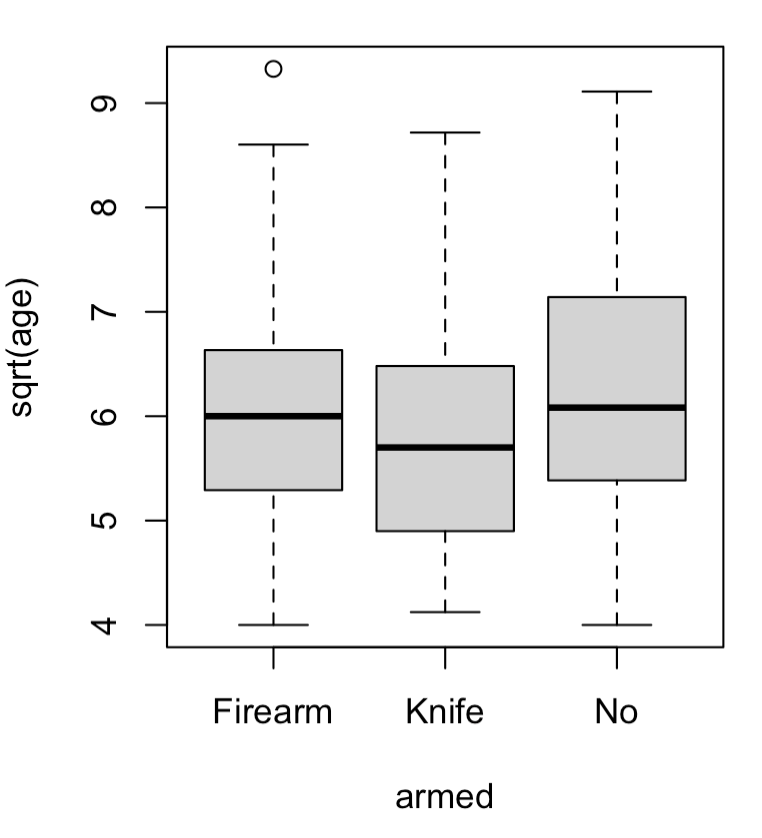
\includegraphics[scale=.35]{boxplot_age_armed.png}
    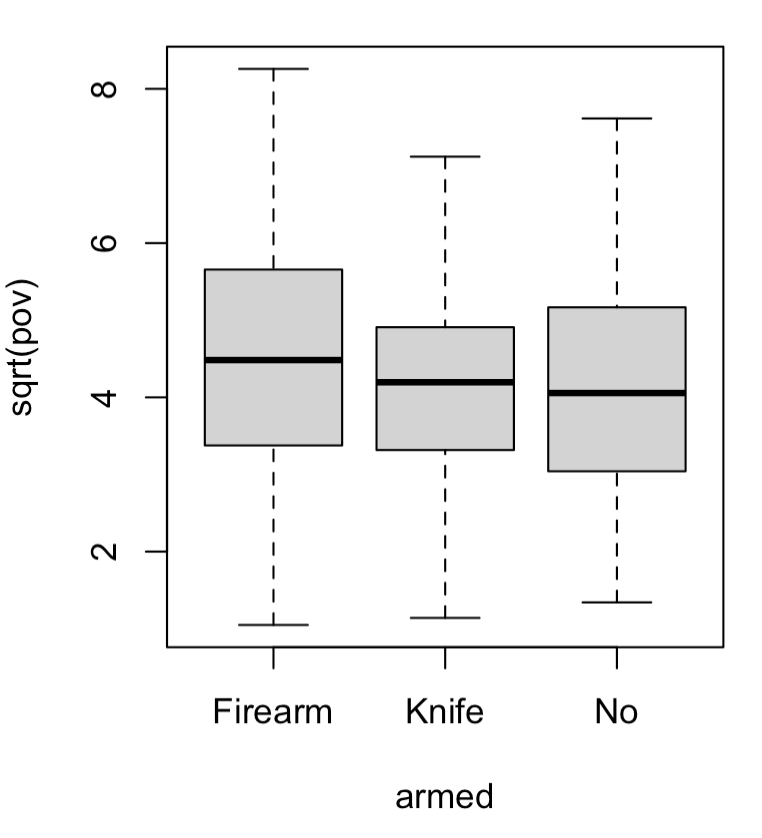
\includegraphics[scale=.35]{boxplot_pov_armed.png}
    \caption{Box plots of $\sqrt{p\_income}$ vs. $raceethnicity$, and of $\sqrt{age}$ and $\sqrt{pov}$ vs. $armed$}
    \label{fig:aov234_boxplots}
\end{figure}

Results for the analysis of $p\_income$ against $raceethnicity$ are summarized in Table \ref{tab:aov2_results}. In this case, Levene's test yields a large $p$-value of 0.417, while Anderson-Darling strongly rejects normality of residuals. The square root transformation is found to worsen variance, so the untransformed model is used this time. Interestingly, the conclusions of our nonparametric tests are considerably stronger than those of our (invalid) parametric tests. The SDCFlig procedure even identifies a significant difference between median age for white vs. Latino victims, which Tukey's HSD does not.

\begin{table}[h]
    \centering
    \begin{tabular}{|l|c|c|c|c|}
        \hline
        \textbf{parameter} & \textbf{procedure} & \textbf{p-value} & \textbf{estimate} & \textbf{95 pct. CI}\\
        \hline
        General & one-way ANOVA & 0.02071 & -- & --\\
        differences & Kruscal-Wallis & 0.0021  & -- & --\\
        \hline
        $\theta_{WB}$ & Tukey's HSD & 0.0428 & $\hat{\mu}_{WB} = 2369.67$ & $(60.56, 4678.77)$\\
        & SDCFlig & 0.0065 & $\hat{\theta}_{WB} = 2657.40$ & $(608.00, 4623.00)$\\
        \hline
        $\theta_{WL}$ & Tukey's HSD & 0.1046 & $\hat{\mu}_{WL} = 2581.70$ & $(-398.68, 5562.09)$\\
        & SDCFlig & 0.0301 & $\hat{\theta}_{WL} = 2520.99$ & $(186.00, 4816.00)$\\
        \hline
        $\theta_{BL}$ & Tukey's HSD & 0.5137 & $\hat{\mu}_{BL} = 212.04$ & $(-3002.64, 3426.71)$\\
        & SDCFlig & 0.9852 & $\hat{\theta}_{BL} = 136.41$ & $(-2747.00, 2529.00)$\\
        \hline
    \end{tabular}
    \caption{Results for $age$ vs. $raceethnicity$}
    \label{tab:aov2_results}
\end{table}

\newpage

\par Our final two analyses involve the categorical variable $armed$. As before, we trim the data to only include the three levels of $armed$ with the most observations. In the resulting dataset, there are 100 unarmed victims, 219 firearm-wielding victims, and 66 knife-wielding victims.

\par \bigskip Table \ref{tab:aov3_results} displays the results of our analysis of $age$ against $armed$. Levene's test again does not reject its null hypothesis for these groups, while the Anderson-Darling test does. The outcomes of the parametric and nonparametric tests in this case are quite similar. One notable difference is that Tukey's HSD returns a much higher $p$-value for $\theta_{FK}$ than for $\theta_{UF}$, while the Kruscal-Wallis $p$-values for those two differences are virtually the same. Perhaps the upper-tailed outliers of age for the firearm- and knife-wielding groups (seen in the second plot in Figure \ref{fig:aov234_boxplots}) make the parametric methods consider those two distributions closer to each other than to the unarmed group.

\vspace{.2in}

\begin{table}[h]
    \centering
    \begin{tabular}{|l|c|c|c|c|}
        \hline
        \textbf{parameter} & \textbf{procedure} & \textbf{p-value} & \textbf{estimate} & \textbf{95 pct. CI}\\
        \hline
        General & one-way ANOVA & 0.0914 & -- & --\\
        differences & Kruscal-Wallis & 0.0796  & -- & --\\
        \hline
        $\theta_{UF}$ & Tukey's HSD & 0.1620 & $\hat{\mu}_{UF} = 2.852$ & $(-0.820, 6.524)$\\
        & SDCFlig & 0.3590 & $\hat{\theta}_{UF} = 2.000$ & $(-2.000, 6.000)$\\
        \hline
        $\theta_{UK}$ & Tukey's HSD & 0.0905 & $\hat{\mu}_{UK} = 4.313$ & $(-0.512, 9.139)$\\
        & SDCFlig & 0.0803 & $\hat{\theta}_{UK} = 4.000$ & $(0.000, 9.000)$\\
        \hline
        $\theta_{FK}$ & Tukey's HSD & 0.7004 & $\hat{\mu}_{FK} = 1.461$ & $(-2.811, 5.734)$\\
        & SDCFlig & 0.3239 & $\hat{\theta}_{FK} = 2.000$ & $(-2.000, 6.000)$\\
        \hline
    \end{tabular}
    \caption{Results for $age$ vs. $armed$}
    \label{tab:aov3_results}
\end{table}

\par Lastly, Table \ref{tab:aov4_results} summarizes results for our analysis of $pov$ against $armed$. The $p$-value of Levene's test is an indecisive 0.05415, but the Anderson-Darling test strongly rejects normality, as usual. Across the board, our distribution-free methods are less confident in rejection than our distribution-based methods. Both ANOVA and the Kruscal-Wallis test reject the null only at levels .1 and above.

\begin{table}[h]
    \centering
    \begin{tabular}{|l|c|c|c|c|}
        \hline
        \textbf{parameter} & \textbf{procedure} & \textbf{p-value} & \textbf{estimate} & \textbf{95 pct. CI}\\
        \hline
        General & one-way ANOVA & 0.0672 & -- & --\\
        differences & Kruscal-Wallis & 0.081 & -- & --\\
        \hline
        $\theta_{UF}$ & Tukey's HSD & 0.1874 & $\hat{\mu}_{UF} = -2.682$ & $(-6.283, 0.919)$\\
        & SDCFlig & 0.2043 & $\hat{\theta}_{UF} = 2.470$ & $(-6.000, 0.900)$\\
        \hline
        $\theta_{UK}$ & Tukey's HSD & 0.8364 & $\hat{\mu}_{UK} = 1.145$ & $(-3.587, 5.877)$\\
        & SDCFlig & 0.9754 & $\hat{\theta}_{UK} = 0.530$ & $(-3.400, 4.600)$\\
        \hline
        $\theta_{FK}$ & Tukey's HSD & 0.0815 & $\hat{\mu}_{FK} = 3.827$ & $(-0.363, 8.012)$\\
        & SDCFlig & 0.1456 & $\hat{\theta}_{FK} = 3.000$ & $(-0.700, 7.200)$\\
        \hline
    \end{tabular}
    \caption{Results for $pov$ vs. $armed$}
    \label{tab:aov4_results}
\end{table}


\section{Conclusion}

\par The nonparametric statistical techniques employed in this paper allow us to make several interesting conclusions about the recipients of deadly force from police in America in 2015. The reader is reminded not to extrapolate the following conclusions beyond the year 2015, and that our data includes the entire population of interest and thus its parameters are technically known. Our estimates of the parameters are not so useful in themselves, but our comparisons of the different populations do reveal whether or not differences between them are significant.

\par \bigskip We estimate that white victims are roughly 7 years older than nonwhite victims on average, and that the distribution of age is tighter around the median for nonwhite victims compared to white victims. We expand this conclusion with analysis of variance methods, determining with 95 percent overall confidence that white victims are typically 4-10 years older than Black victims and 5-12 years older than Latino victims, and that there is no meaningful difference in median age between Black and Latino victims. All our conclusions for this variable pair are very strong, so each nonparametric test came to the same conclusion as its parametric counterpart. However, the nonparametric conclusions are more useful because they are much more robust.

\par \bigskip We also estimate with 95 percent confidence that armed victims are between 0 and 6 years younger than unarmed victims on average. We find with a significance level of .1 that unarmed victims are between 0 and 9 years older than knife-wielding victims on average. On the other hand, we find no differences in the distributions of tract-level poverty rate based on whether or not the victim was armed, nor based on whether the victim specifically wielded a firearm, a knife, or no weapon. Nonparametric methods generally yield more conservative $p$-values in these analyses, but the Miller jackknife procedure comes closer to rejecting the null hypothesis of equal dispersion.

\par \bigskip Finally, we find with 95 percent confidence that, on average, white victims were killed in tracts with average personal incomes between \$608 and \$4623 higher than in the tracts of Black victims, and between \$186 and \$4816 higher than in the tracts of Latino victims. Distribution-free techniques prove considerably more confident than their counterparts for this pair of variables.

\par \bigskip Throughout our analyses, the nonparametric procedures proved to be resilient to both outliers and atypical distribution variances compared to their parametric cousins. Our data provided good examples of how transformations are unnecessary for rank-based nonparametric tests, giving them an advantage in this setting.

\newpage

\subsection{Further Discussion}

\par \bigskip Our conclusions point to other worthwhile investigations using these data. One interesting thread to pull would be how closely the victim population represents the general population. For instance, to look for significant racial disparities, one could group victims geographically and compare the racial proportions to the general population of each area using variables like $share\_white$, $share\_black$, and $share\_hispanic$. There is certainly no way to design an ethical experiment about police use of deadly force, so future analysis would have to remain in the realm of relations without making inferences about causations.

\begin{thebibliography}{99}
    \bibitem{dset} B. Casselman, ``Where Police Have Killed Americans In 2015." \textit{FiveThirtyEight}, June 3, 2015. Retrieved December 14, 2021 from https://fivethirtyeight.com/features/where-police-have-killed-americans-in-2015/. Dataset: FiveThirtyEight Police Killings, Version 105. Retrieved December 14, 2021 from https://www.kaggle.com/fivethirtyeight/fivethirtyeight-police-killings-dataset/version/105.
\end{thebibliography}

\end{document}
